%% monografia.tex, fabiokepler, jeancheiran
%% Copyright 2012-2018 by UNIPAMPA LaTeX group at https://bitbucket.org/unipampaalegrete/monografias-cc-es-repo/
%%
%% This work may be distributed and/or modified under the conditions of the LaTeX Project Public
%% License, either version 1.3 of this license or (at your option) any later version.
%% The latest version of this license is in
%%   http://www.latex-project.org/lppl.txt
%% and version 1.3 or later is part of all distributions of LaTeX version 2005/12/01 or later.
%%
%% Based on the example file abtex2-modelo-trabalho-academico.tex of the abntex2 package
%% (http://abntex2.googlecode.com/) and on the ppgccufmg 1.45beta2 class
%% (http://vilarneto.com/ppgccufmg,
%% http://www.dcc.ufmg.br/pos/alunos/modelodisstese.php
%% and http://www.dcc.ufmg.br/~mirella).
%%
%% Adapted for the Computer Science program at UNIPAMPA (http://www.unipampa.edu.br)
%% by Fabio Kepler (fabio@kepler.pro.br) and Jean Cheiran (jeancheiran@unipampa.edu.br).
%%
%% Version 2.5 - 2018/08
%% Version 2.4 - 2017/05
%% Version 2.3 - 2013/03

% +++++++++++++++++++++++++++++++++++++++++++++++++++++++++++++++++++++++++++++++++++++++++++++++++
% Este modelo utiliza o pacote abnTeX2. Veja como instalá-lo em seu ambiente em
% http://abntex2.googlecode.com/.
% -------------------------------------------------------------------------------------------------
% abnTeX2: Modelo de Trabalho Acadêmico (tese de doutorado, dissertação de
% mestrado e trabalhos monográficos em geral) em conformidade com
% ABNT NBR 14724:2011: Informação e documentação - Trabalhos acadêmicos -
% Apresentação
% -------------------------------------------------------------------------------------------------
% Normas institucionais utilizadas:
% http://porteiras.r.unipampa.edu.br/portais/sisbi/programa-de-capacitacao/
% +++++++++++++++++++++++++++++++++++++++++++++++++++++++++++++++++++++++++++++++++++++++++++++++++

\documentclass[12pt,openright,twoside,a4paper,chapter=TITLE]{abntex2}    % frente e verso
%\documentclass[12pt,oneside,a4paper]{abntex2}            % apenas frente

% +++++++++++++++++++++++++++++++++++++++++++++++++++++++++++++++++++++++++++++++++++++++++++++++++
% PACOTES
% -------------------------------------------------------------------------------------------------
% Pacotes fundamentais
\usepackage{cmap}           % Mapeamento de caracteres especiais no PDF
\usepackage{lmodern}        % Usa fonte Latin Modern
\usepackage[T1]{fontenc}    % Seleção de codificação de fonte
\usepackage[utf8]{inputenc} % Codificação do arquivo (conversão automática dos acentos)
\usepackage[brazil]{babel}  % Idioma para hifenização e tradução de vários elementos
\usepackage{makeidx}        % Criação de índice
\usepackage{hyperref}       % Formatação do índice
\usepackage{lastpage}       % Usado pela Ficha catalográfica
\usepackage{indentfirst}    % Indenta o primeiro parágrafo de cada seção
\usepackage[usenames,dvipsnames]{xcolor}  % Controle das cores (com nomes)
\usepackage{graphicx}       % Inclusão de gráficos
\usepackage{booktabs}       % Formatação de tabelas
% -------------------------------------------------------------------------------------------------
% Para citações
\usepackage[brazilian,hyperpageref]{backref} % Páginas com as citações na bibliografia
\usepackage[alf,abnt-emphasize=bf]{abntex2cite} % Citações padrão ABNT (alfanumérico)
% -------------------------------------------------------------------------------------------------
% Pacotes opcionais
\usepackage{nomencl}        % Para criar uma lista de símbolos
\usepackage{acro}           % Para usar acrônimos e abreviaturas
\usepackage{tikz}           % Para fazer figuras, diagramas e gráficos integrados e elegantes
\usepackage{pgfplots}       % Usa o pacote tikz para fazer gráficos muito melhores que os do Excel
\usepackage{pgfplotstable}  % Para gerar tabelas automaticamente a partir de arquivos com dados
\usepackage{filecontents}   % Para colocar o conteúdo de um arquivo dentro de um arquivo tex
\usepackage{todonotes}      % Para criar anotações durante o desenvolvimento do texto
%\usepackage{multirow}       % Permite fazer tabelas com múltiplas linhas
%\let\newfloat=\undefined    % Workaround para usar o pacote algorithm
%\usepackage{algorithm}      % Para escrever algoritmos
%\usepackage{clrscode}       % Para escrever algoritmos
%\usepackage{clrscode3e}     % Para escrever algoritmos; mais simples que os pacotes acima
\usepackage{pdfpages}        % Para incluir a folha de aprovação assinada em PDF
% -------------------------------------------------------------------------------------------------
% Configurações de pacotes
% -------------------------------------------------------------------------------------------------
\addto\captionsbrazil{
  \renewcommand{\listfigurename}{Lista de figuras}
}
% -------------------------------------------------------------------------------------------------
% Configurações do pacote backref
% Usado sem a opção hyperpageref de backref
\renewcommand{\backrefpagesname}{Citado na(s) página(s):~}
% Texto padrão antes do número das páginas
\renewcommand{\backref}{}
% Define os textos da citação
\renewcommand*{\backrefalt}[4]{
    \ifcase #1 %
        Nenhuma citação no texto.%
    \or
        Citado na página #2.%
    \else
        Citado #1 vezes nas páginas #2.%
    \fi}%
% -------------------------------------------------------------------------------------------------
% Configurações de aparência do PDF final
%\definecolor{blue}{RGB}{41,5,195}
% \definecolor{webgreen}{rgb}{0,.5,0}
% Metainformações do PDF e cores dos links
\hypersetup{
  portuguese,
  %backref=true,
  %pagebackref=true,
  %bookmarks=true,             % show bookmarks bar?
  %bookmarksnumbered=true,
  bookmarksdepth=4,
  pdftitle={\@title},
  pdfauthor={\@author},
  pdfsubject={\imprimirpreambulo},
  pdfkeywords={UNIPAMPA}{Computação}{UNIPAMPA}{abntex}{TCC},
  %pdfproducer={LaTeX with abnTeX2},     % producer of the document
  pdfcreator={\@author},
  colorlinks=true,           % false: boxed links; true: colored links
  linkcolor=black,            % color of internal links
  citecolor=black,            % color of links to bibliography
  filecolor=black,         % color of file links
  urlcolor=black
}
%   linktocpage,
%   colorlinks,
%   citecolor=webgreen,
%   urlcolor=Maroon,
%   linkcolor=RoyalBlue,
%   filecolor=black,
% -------------------------------------------------------------------------------------------------
% Espaçamentos entre linhas e parágrafos
% O tamanho do parágrafo é dado por
\setlength{\parindent}{1.3cm}
% Controle do espaçamento entre um parágrafo e outro
\setlength{\parskip}{0.2cm} % tente também \onelineskip
% Controles do espaçamento entre linhas
%\OnehalfSpacing       % espaçamento um e meio (padrão);
%\DoubleSpacing        % espaçamento duplo
%\SingleSpacing        % espaçamento simples
% -------------------------------------------------------------------------------------------------
% Para o pacote de acrônimos
\acsetup{hyperref=true,index=true} %first-style=short}
% -------------------------------------------------------------------------------------------------
% Para o pacote tikz, pgfplots e pgfplotstable
\usetikzlibrary{arrows,chains,matrix,positioning,decorations.pathreplacing,calc}
% -------------------------------------------------------------------------------------------------
% Para poder usar subfiguras e subtabelas
\newsubfloat{figure}
\newsubfloat{table}
\providecommand*{\subfigureautorefname}{\figureautorefname}
% +++++++++++++++++++++++++++++++++++++++++++++++++++++++++++++++++++++++++++++++++++++++++++++++++


% +++++++++++++++++++++++++++++++++++++++++++++++++++++++++++++++++++++++++++++++++++++++++++++++++
% Informações de dados para CAPA e FOLHA DE ROSTO
% -------------------------------------------------------------------------------------------------
\titulo{Modelo para Trabalho de Conclusão de Curso}
\autor{Nome do autor}
\local{Alegrete}
\data{2017}
\orientador{Prof. <titulação> Nome do Orientador}
\coorientador{Prof. <titulação> Nome do Coorientador} % Se houver
\instituicao{Universidade Federal do Pampa}
%\tipotrabalho{Projeto de Trabalho de Conclusão de Curso~} % Para TCC I
\tipotrabalho{Trabalho de Conclusão de Curso~} % Para TCC II
% O preambulo deve conter o tipo do trabalho, o objetivo, o nome da instituição e a área de concentração
\preambulo{\imprimirtipotrabalho apresentado ao Curso de Graduação em Ciência da
           Computação da Universidade Federal do Pampa como requisito parcial para a obtenção do
           título de Bacharel em Ciência da Computação.}
% +++++++++++++++++++++++++++++++++++++++++++++++++++++++++++++++++++++++++++++++++++++++++++++++++

% -------------------------------------------------------------------------------------------------
% Compila o indice
\makeindex
% Compila a lista de abreviaturas e siglas
% Para funcionar, o seguinte comando deve ser executado:
% makeindex ARQUIVO_PRINCIPAL.nlo -s nomencl.ist -o ARQUIVO_PRINCIPAL.nls
\makenomenclature
% -------------------------------------------------------------------------------------------------

% -------------------------------------------------------------------------------------------------
% Abreviaturas (definido pelo parâmetro 'class')
\DeclareAcronym{fig}{
  short = Fig.,
  long  = Figura,
  class = abreviaturas
}
% -------------------------------------------------------------------------------------------------
% Acrônimos/Siglas (definido pelo parâmetro 'class')
\DeclareAcronym{tcc}{
  short = TCC,
  long  = Trabalho de Conclusão de Curso,
  long-plural-form = Trabalhos de Conclusão de Curso,
  class = acronimos
}
% -------------------------------------------------------------------------------------------------
% Nomenclaturas/Símbolos
\nomenclature{$A_i$}{Área do $i^{esimo}$ componente}
\nomenclature{456}{Isto é um número}
\nomenclature{123}{Isto é outro número}
\nomenclature{$n$}{Tamanho da entrada}
\nomenclature{$V$}{Vetor de elementos}
\nomenclature{$\mathcal{T}$}{Conjunto de trabalhos de TCC}

% -------------------------------------------------------------------------------------------------
% Inclui alguns ajustes finos para que fique de acordo com o Manual de Normatização
% Pequenos consertos e ajustes para que fique de acordo com o Manual de Normatização 2011.

\setlength{\ABNTEXsignwidth}{12cm}

% ---
% Impressão da Capa
\renewcommand{\imprimircapa}{%
  \begin{capa}%
    \center
    {\ABNTEXchapterfont\large\MakeUppercase\imprimirinstituicao}

    \vspace*{\fill}
    {\ABNTEXchapterfont\large\imprimirautor}

    \vspace*{\fill}
    {\ABNTEXchapterfont\bfseries\LARGE\imprimirtitulo}

    \vspace*{\fill}
    ~
    \vspace*{\fill}

    {\large\imprimirlocal}
    \par
    {\large\imprimirdata}

    \vspace*{1cm}
  \end{capa}
}
% ---


% ---
% Impressão da Folha de Rosto
\makeatletter
\renewcommand{\folhaderostocontent}{
  \begin{center}

    {\ABNTEXchapterfont\large\imprimirautor}

    \vspace*{\fill}%\vspace*{\fill}
    {\ABNTEXchapterfont\bfseries\Large\imprimirtitulo}
    \vspace*{\fill}

    \abntex@ifnotempty{\imprimirpreambulo}{%
      \hspace{.45\textwidth}
      \begin{minipage}{.5\textwidth}
        {\SingleSpacing
        \imprimirpreambulo}

        \vspace*{1em}
        \imprimirorientadorRotulo~\imprimirorientador\par

        \abntex@ifnotempty{\imprimircoorientador}{%
          \vspace*{1em}
          \imprimircoorientadorRotulo~\imprimircoorientador%
        }%

      \end{minipage}%
      \vspace*{\fill}
    }%

    {\large\imprimirlocal}
    \par
    {\large\imprimirdata}
    \vspace*{1cm}

  \end{center}
}
\makeatother
% ---

% ---
\renewcommand{\ABNTEXchapterfont}{\rmfamily\bfseries}
\setsecheadstyle{\rmfamily\bfseries}

\renewcommand{\ABNTEXchapterfontsize}{\normalsize}
\renewcommand{\ABNTEXsectionfontsize}{\normalsize}
\renewcommand{\ABNTEXsubsectionfontsize}{\normalsize}
\renewcommand{\ABNTEXsubsubsectionfontsize}{\normalsize}
\renewcommand{\ABNTEXsubsubsubsectionfontsize}{\normalsize}

% Espaçamento entre título e texto
\setlength\afterchapskip{\lineskip}

% Espaçamento entre parágrafos
\setlength{\parskip}{0.cm}

% ---




% *************************************************************************************************
\begin{document}
% *************************************************************************************************

% +++++++++++++++++++++++++++++++++++++++++++++++++++++++++++++++++++++++++++++++++++++++++++++++++
% ELEMENTOS PRÉ-TEXTUAIS
% +++++++++++++++++++++++++++++++++++++++++++++++++++++++++++++++++++++++++++++++++++++++++++++++++
% \pretextual

% -----------------------------------------------
% Capa [OBRIGATÓRIO]
% -----------------------------------------------
\imprimircapa

% -----------------------------------------------
% Folha de rosto [OBRIGATÓRIO]
% -----------------------------------------------
% (ver documentação do abntex2 caso seja necessário haver ficha catalográfica)
\imprimirfolhaderosto

% -----------------------------------------------
% Folha de aprovação [OBRIGATÓRIO]
% -----------------------------------------------
% Veja alguns detalhes no arquivo.
% -----------------------------------------------
% Folha de aprovação [OBRIGATÓRIO]
% -----------------------------------------------
% Este é um exemplo de Folha de aprovação, elemento obrigatório da NBR 14724/2011 (seção 4.2.1.3).
% Você pode utilizar este modelo até a aprovação do trabalho.
% Após isso, altere o conteúdo deste arquivo para inserir uma imagem da página assinada pela banca usando
% o modelo que está no final deste arquivo.

% -----------------------------------------------
% Folha de aprovação antes da defesa do TCC
% -----------------------------------------------
%\begin{comment}
\begin{folhadeaprovacao}
  \begin{center}
    {\ABNTEXchapterfont\large\imprimirautor}

    \vspace*{\fill}%\vspace*{\fill}
    {\ABNTEXchapterfont\bfseries\Large\imprimirtitulo}
    \vspace*{\fill}

    \hspace{.45\textwidth}
    \begin{minipage}{.5\textwidth}
        \imprimirpreambulo
    \end{minipage}%
    \vspace*{\fill}
  \end{center}

  \begin{center}
    \imprimirtipotrabalho defendido e aprovado em ..... de .............. de ......

    Banca examinadora:
  \end{center}

  \assinatura{\textbf{\imprimirorientador} \\ Orientador \\ <sigla da instituição>}
  \makeatletter
  \abntex@ifnotempty{\imprimircoorientador}{%
    \assinatura{\textbf{\imprimircoorientador} \\ Coorientador \\ <sigla da instituição>}%
  }
  \makeatother
  \assinatura{\textbf{Prof. <titulação> Nome Professor} \\ <sigla da instituição>}
  \assinatura{\textbf{Prof. <titulação> Nome Professor} \\ <sigla da instituição>}

\end{folhadeaprovacao}
%\end{comment}
% -----------------------------------------------
% Folha de aprovação após a defesa do TCC com a imagem da folha de aprovação assinada pela banca.
% -----------------------------------------------
\begin{comment}
\begin{folhadeaprovacao}

% Escolher entre uma das seguintes opções para inclusão da folha de aprovação
% Versão assinada em arquivo PDF (incluir no arquivo principal o comando \usepackage{pdfpages})
%\includepdf{pretextuais/aprovacao.pdf}

% Ou, versão assinada em arquivo de imagem (jpg, png, etc)
% Mas prefira em PDF. Em imagem é preciso acertar os recuos das margens:
%\vspace*{-4cm}
%\hspace*{-3.5cm}
%\includegraphics[width=\paperwidth]{pretextuais/aprovacao}

\end{folhadeaprovacao}
\end{comment}


% -----------------------------------------------
% Dedicatória [OPCIONAL]
% -----------------------------------------------
\begin{dedicatoria}
   \vspace*{\fill}
   \begin{flushright}
     Este trabalho é dedicado às crianças adultas que,\\
     quando pequenas, sonharam em se tornar cientistas.
   \end{flushright}
   \vspace*{\fill}
\end{dedicatoria}


% -----------------------------------------------
% Agradecimentos [OPCIONAL]
% -----------------------------------------------
\begin{agradecimentos}

Sed ut perspiciatis unde omnis iste natus error sit voluptatem accusantium doloremque laudantium, totam rem aperiam, eaque ipsa quae ab illo inventore veritatis et quasi architecto beatae vitae dicta sunt explicabo. Nemo enim ipsam voluptatem quia voluptas sit aspernatur aut odit aut fugit, sed quia consequuntur magni dolores eos qui ratione voluptatem sequi nesciunt. Neque porro quisquam est, qui dolorem ipsum quia dolor sit amet, consectetur, adipisci velit, sed quia non numquam eius modi tempora incidunt ut labore et dolore magnam aliquam quaerat voluptatem. Ut enim ad minima veniam, quis nostrum exercitationem ullam corporis suscipit laboriosam, nisi ut aliquid ex ea commodi consequatur? Quis autem vel eum iure reprehenderit qui in ea voluptate velit esse quam nihil molestiae consequatur, vel illum qui dolorem eum fugiat quo voluptas nulla pariatur?

At vero eos et accusamus et iusto odio dignissimos ducimus qui blanditiis praesentium voluptatum deleniti atque corrupti quos dolores et quas molestias excepturi sint occaecati cupiditate non provident, similique sunt in culpa qui officia deserunt mollitia animi, id est laborum et dolorum fuga. Et harum quidem rerum facilis est et expedita distinctio. Nam libero tempore, cum soluta nobis est eligendi optio cumque nihil impedit quo minus id quod maxime placeat facere possimus, omnis voluptas assumenda est, omnis dolor repellendus. Temporibus autem quibusdam et aut officiis debitis aut rerum necessitatibus saepe eveniet ut et voluptates repudiandae sint et molestiae non recusandae. Itaque earum rerum hic tenetur a sapiente delectus, ut aut reiciendis voluptatibus maiores alias consequatur aut perferendis doloribus asperiores repellat.

\end{agradecimentos}

% -----------------------------------------------
% Epígrafe [OPCIONAL]
% -----------------------------------------------
\begin{epigrafe}
  \vspace*{\fill}
	\begin{flushright}
		``Não vos amoldeis às estruturas deste mundo, \\
		mas transformai-vos pela renovação da mente, \\
		a fim de distinguir qual é a vontade de Deus: \\
		o que é bom, o que Lhe é agradável, o que é perfeito.\\
		(Bíblia Sagrada, Romanos 12:2)
	\end{flushright}
\end{epigrafe}


% -----------------------------------------------
% Resumo [OBRIGATÓRIO]
% -----------------------------------------------
\begin{resumo}
 Segundo a \citeonline[3.1-3.2]{NBR6028:2003}, o resumo deve ressaltar o
 objetivo, o método, os resultados e as conclusões do documento. A ordem e a extensão
 destes itens dependem do tipo de resumo (informativo ou indicativo) e do
 tratamento que cada item recebe no documento original. O resumo deve ser
 precedido da referência do documento, com exceção do resumo inserido no
 próprio documento. (\ldots) As palavras-chave devem figurar logo abaixo do
 resumo, antecedidas da expressão Palavras-chave:, separadas entre si por
 ponto e finalizadas também por ponto.

 \vspace{\onelineskip}
    
 \noindent
 \textbf{Palavras-chave}: Aprendizado de Máquina. Linguística Computacional. Sabotagens.
\end{resumo}


% -----------------------------------------------
% Abstract (resumo em inglês) [OBRIGATÓRIO]
% -----------------------------------------------
\begin{resumo}[Abstract]
 This is the english abstract.

 \vspace{\onelineskip}
 
 \noindent 
 \textbf{Key-words}: Machine Learning. Computational Linguistics. Sabotage.
\end{resumo}


% Resumo estendido [OPCIONAL]
% \input{pretextuais/resumoest}

% -----------------------------------------------
% Listas
% -----------------------------------------------
% Figuras/Ilustrações [OPCIONAL]
\pdfbookmark[0]{\listfigurename}{lof}
\listoffigures*
\cleardoublepage
% -----------------------------------------------
% Tabelas [OPCIONAL]
\pdfbookmark[0]{\listtablename}{lot}
\listoftables*
\cleardoublepage
% -----------------------------------------------
% Abreviaturas [OPCIONAL] (veja o pacote acro e os exemplo acima)
\newcommand{\lobname}{Lista de abreviaturas}
\pdfbookmark[0]{\lobname}{lob}
\printacronyms[include-classes=abreviaturas,name=\lobname,heading=chapter*]
\cleardoublepage
% -----------------------------------------------
% Siglas [OPCIONAL] (veja o pacote acro e os exemplo acima)
\newcommand{\loaname}{Lista de siglas}
\pdfbookmark[0]{\loaname}{loa}
\printacronyms[include-classes=acronimos,name=\loaname,heading=chapter*]
\cleardoublepage
% -----------------------------------------------
% Símbolos [OPCIONAL] (veja o pacote nomencl e os exemplo acima)
\renewcommand{\nomname}{Lista de símbolos}
\pdfbookmark[0]{\nomname}{los}
\printnomenclature
\cleardoublepage


% -----------------------------------------------
% Sumário
% -----------------------------------------------
\pdfbookmark[0]{\contentsname}{toc}
\tableofcontents*
\cleardoublepage
% -----------------------------------------------

\begin{comment}
  %cutter={M1234x}, % INFORMAÇÃO QUE VAI NA FICHA CATALOGRÁFICA
  %cdu={100.0*01.10},  % Define o identificador CDU do documento, fornecido pela Secretaria do Curso (verificar se é necessário).
  keywords={Modelo de texto, UNIPAMPA, Latex}, % Define as palavras-chave que deverão constar na Ficha Catalográfica, separadas por vírgulas.
  firstcommitteemember={Nome membro da banca 1\\ UNIPAMPA},
  secondcommitteemember={Nome membro da banca 2\\ Instituição},
\end{comment}



% +++++++++++++++++++++++++++++++++++++++++++++++++++++++++++++++++++++++++++++++++++++++++++++++++
% ELEMENTOS TEXTUAIS
% +++++++++++++++++++++++++++++++++++++++++++++++++++++++++++++++++++++++++++++++++++++++++++++++++
% É possível usar \textual ou \mainmatter, que é a macro padrão do memoir.
\textual

% Você pode dividir o seu texto em vários arquivos. Por exemplo, um para cada seção principal do
% trabalho: introducao.tex, relacionados.tex, metodologia.tex, experimentos.tex, conclusao.tex.
%==============================================================================
\chapter{Introdução}\label{introducao}
%==============================================================================

Este trabalho mostra alguns exemplos de utilização de comandos \LaTeX, opções de formatação e dicas de conteúdo.
  Várias partes foram retiradas do manual da classe \abnTeX~\cite{abntex2classe,abntex2cite}, e algumas partes, principalmente o anexo \ref{anexo:latex}, de \cite{Moro2012}.
  A propósito, recomenda-se a leitura de \cite{Moro2012}, pois contém dicas de como escrever um trabalho de pós-graduação que podem ser aplicadas também a \acp{tcc}.
  Leia também \cite{SisbiUnipampa2011} para mais informações sobre como escrever um trabalho.


%------------------------------------------------------------------------------
\section{Divisões do documento: seção}\label{sec:divisoes}
%------------------------------------------------------------------------------

Esta seção testa o uso de divisões de documentos. Isto é uma seção.


%------------------------------------------------------------------------------
\subsection{Divisões do documento: subseção}
%------------------------------------------------------------------------------

Isto é uma subseção.


%------------------------------------------------------------------------------
\subsubsection{Divisões do documento: subsubseção}
%------------------------------------------------------------------------------

Isto é uma subsubseção.


%------------------------------------------------------------------------------
\subsubsection{Divisões do documento: subsubseção}
%------------------------------------------------------------------------------

Isto é outra subsubseção.


%------------------------------------------------------------------------------
\subsection{Divisões do documento: subseção}\label{sec:exemplo-subsec}
%------------------------------------------------------------------------------

Isto é uma subseção.


%------------------------------------------------------------------------------
\subsubsection{Divisões do documento: subsubseção}
%------------------------------------------------------------------------------

Isto é mais uma subsubseção da \autoref{sec:exemplo-subsec}.


%------------------------------------------------------------------------------
\section{Este é um exemplo de nome de seção longo. Ele deve estar alinhado à esquerda e a segunda e demais linhas devem iniciar logo abaixo da primeira palavra da primeira linha}
%------------------------------------------------------------------------------

Isso atende à norma \citeonline[seções de 5.2.2 a 5.2.4]{NBR14724:2011} e \citeonline[seções de 3.1 a 3.8]{NBR6024:2012}.


%------------------------------------------------------------------------------
\section{Consulte o manual da classe \textsf{abntex2}}
%------------------------------------------------------------------------------

Consulte o manual da classe \textsf{abntex2} \cite{abntex2classe} para uma referência completa das macros e ambientes disponíveis.
  Além disso, o manual possui informações adicionais sobre as normas ABNT observadas pelo \abnTeX.


%------------------------------------------------------------------------------
\section{Organização deste trabalho}
%------------------------------------------------------------------------------

No \autoref{desenvolvimento} há várias instruções e dicas de uso deste modelo, e o \autoref{anexo:latex}\todo{BUG do abntex2: deveria referenciar como Anexo.}~traz dicas sobre o uso do \LaTeX.
 % [OBRIGATORIO]
%\part{Revisão de Literatura} % Pode-se usar partes para organizar os capítulos
%==============================================================================
\chapter{Desenvolvimento}\label{desenvolvimento}
%==============================================================================

Alguns cuidados devem ser tomados no uso deste pacote.
  Leia as orientações a seguir e contate o responsável em caso de dúvidas.


%------------------------------------------------------------------------------
\section{Formatação}
%------------------------------------------------------------------------------

Embora não faça diferença no resultado final, é importante formatar adequadamente o seu código \LaTeX.
  Da mesma forma que para outras linguagens de programação, isso aumenta a legibilidade do código e ajuda a encontrar partes específicas mais rapidamente.
  As principais dicas para arquivos \TeX são:
 \begin{itemize}
   \item Indente seu código. Não só os ambientes (begin, end) mas também os parágrafos! Coloque cada sentença em uma linha, indentando a partir da segunda;
   \item Coloque marcações comentadas para delimitar o início de capítulos, seções, etc. Isso facilita buscar partes específicas em um arquivo.
 \end{itemize}

Cuidado com abreviaturas e acrônimos.
  É fácil esquecer de os definir ou definir de maneira diferente em capítulos diferentes.
  Use os comandos do pacote \texttt{acro} para abreviaturas e acrônimos.
  Por exemplo, \ac{fig} é uma abreviação, então \ac{tcc} é um acrônimo/sigla.
  Eles são definidos no preâmbulo do documento.

Também vale a pena usar uma tabela de nomenclatura caso você use muitos símbolos, em especial símbolos matemáticos.
  Veja os comandos do pacote \texttt{nomencl}.
  As definições também ficam no preâmbulo do documento.


%------------------------------------------------------------------------------
\section{Codificação dos arquivos: UTF8}
%------------------------------------------------------------------------------

A codificação de todos os arquivos deste pacote é \texttt{UTF8}.
  É necessário que você utilize a mesma codificação nos documentos que escrever, inclusive nos arquivos de bases bibliográficas |.bib|.


%------------------------------------------------------------------------------
\section{Citações}
%------------------------------------------------------------------------------

\index{citações!diretas}Utilize o ambiente \texttt{citacao} para incluir citações diretas com mais de três linhas:

\begin{citacao}
As citações diretas, no texto, com mais de três linhas, devem ser destacadas com recuo de 4 cm da margem esquerda, com letra menor que a do texto utilizado e sem as aspas.
  No caso de documentos datilografados, deve-se observar apenas o recuo \cite[5.3]{NBR10520:2002}
\end{citacao}

\index{citações!simples}Citações simples, com até três linhas, devem ser incluídas com aspas.
  Observe que em \LaTeX~as aspas iniciais são diferentes das finais: ``Amor é fogo que arde sem se ver''.

Para as citações indiretas, o comando padrão, \verb|\cite|, realiza a forma mais comum de citação \cite{SisbiUnipampa2011}.
  A outra das formas mais usadas, para citar em texto corrido, é conseguida com o comando \verb|\citeonline|: segundo \citeonline{SisbiUnipampa2011}, na citação indireta, o número da página é opcional.


%------------------------------------------------------------------------------
\subsection{Referências internas}\label{sec:referencias_internas}
%------------------------------------------------------------------------------

Usa-se o comando \verb|\ref{}| para referenciar uma Tabela ou Figura.
  Por exemplo, esta é uma referência para a Tabela~\ref{tab:nivinv}.
  Mas também pode-se usar o comando \verb|\autoref{}|, que insere o tipo também.
  Por exemplo, esta é outra referência para a \autoref{tab:nivinv}.

Há vários outros comandos interessantes.
  Eles estão no fonte do \autoref{introducao}, na \autoref{sec:referencias_internas}
  \footnote{O número do capítulo indicado é \ref{introducao}, que se inicia à página \pageref{introducao}.}
  (\nameref{introducao}, \autopageref{introducao}).


%------------------------------------------------------------------------------
\section{Tabelas}
%------------------------------------------------------------------------------

\index{tabelas}A \autoref{tab:nivinv} é um exemplo de tabela construída em \LaTeX.
  Como sugestão de formatação, evite ao máximo o uso de linhas verticais.
  As colunas de uma tabela devem ser separadas visivelmente.
  O contrário indica que a tabela está mal formatada ou que certas informações não deveriam estar nela.

Da mesma forma, evite o uso de linhas horizontais para separar linhas da tabela.
  Use-as apenas para separar o cabeçalho e eventuais partes importantes.
  Para obter um resultado ainda mais elegante, use os comandos do pacote \texttt{booktabs}.

Veja essas sugestões aplicas na \autoref{tab:nivinv}.

\begin{table}[!htb]
\footnotesize
\caption[Níveis de investigação]{Níveis de investigação.}
\label{tab:nivinv}
\begin{tabular}{m{2.6cm}m{6.0cm}m{2.25cm}m{3.40cm}}
  \toprule
  \textbf{Nível de Investigação} & \textbf{Insumos}  & \textbf{Sistemas de Investigação}  & \textbf{Produtos}  \\
  \midrule
  Meta-nível & Filosofia\index{filosofia} da Ciência  & Epistemologia & Paradigma  \\
  Nível do objeto & Paradigmas do metanível e evidências do nível inferior & Ciência  & Teorias e modelos \\
  Nível inferior & Modelos e métodos do nível do objeto e problemas do nível inferior & Prática & Solução de problemas  \\
  \bottomrule
\end{tabular}
\fonte{\citeonline{van86}}
\end{table}


Uma opção avançada para a criação de tabelas é usar o pacote \texttt{pgfplotstable}.
  Ele permite que os dados de um arquivo sejam lidos e colocados em uma tabela, formatando-os da maneira que se quiser.
  A \autoref{tab:dados} é um exemplo.
  Veja o arquivo \texttt{desenvolvimento.tex} para os comandos necessários.

% Necessário o pacote filecontents
% Especifica o conteúdo que será gravado no dado arquivo (nesse caso, resultados.txt)
\begin{filecontents*}{resultados.txt}
tamanho metodo1 metodo2 metodo3
10  30    36.2  28.3
20  54.8  52.5  56.8
30  65    59.6  74.1
40  64.5  59.6  76.7
50  64.6  59.6  76.5
\end{filecontents*}

% Para definir os estilos das colunas e da tabela
\pgfplotstableset{
     %columns={tamanho,metodo1,{grad(log(metodo2),log(metodo3))}},
     columns/metodo1/.style={
         column name=\textsc{Método 1 (\%)},
         column type=c,
         %dec sep align={c},
         %sci,sci zerofill,sci subscript,
         fixed,fixed zerofill,
         precision=1},
     columns/metodo2/.style={
         column name=\textsc{Método 2 (\%)},
         column type=c,
         fixed,fixed zerofill,precision=1},
     columns/metodo3/.style={
         column name=\textsc{Método 3 (\%)},
         fixed,fixed zerofill,precision=1},
     columns/media/.style={
         column name=\textsc{Média (\%)},
         fixed,fixed zerofill,precision=1},
     create on use/media/.style={
         create col/expr={(\thisrow{metodo1}+\thisrow{metodo2}+\thisrow{metodo3})/3}},
     every head row/.style={
         before row=\toprule,after row=\midrule},
     every last row/.style={
         after row=\bottomrule}}

\begin{table}[!phtb]
  \caption{Exemplo de tabela com dados de arquivo.}
  \label{tab:dados}
  \begin{center}
    % Lê do arquivo resultados.txt as colunas especificadas e as formata de acordo com
    % os estilos acima ou com os estilos especificados aqui (nesse caso, para a coluna tamanho).
    \pgfplotstabletypesetfile[
      columns={tamanho,metodo1,metodo2,metodo3,media},
      columns/tamanho/.style={column name=\textsc{Tamanho}}
    ]{resultados.txt}
  \end{center}
\end{table}


%------------------------------------------------------------------------------
\section{Figuras}
%------------------------------------------------------------------------------

\index{figuras}Figuras podem ser criadas diretamente em \LaTeX.
  Uma das melhores formas, por ser relativamente simples, bem documentada e gerar ótimos resultados, é com o uso do pacote tikz\footnote{Há vários exemplos em \url{http://www.texample.net/}.}.
  Ele permite gerar diagramas, árvores, fluxogramas etc.
  A \autoref{fig:fib} mostra um exemplo simples de árvore.

\begin{figure}[!htb]
  \caption{Árvore de recursão de Fibonacci.}\label{fig:fib}
  \begin{center}
  \begin{tikzpicture}[level/.style={sibling distance=160mm/(2^#1)},
                      level 4/.style={sibling distance=18mm},
                      every node/.style={minimum width=5mm}]
    \node [circle,draw] (z) {$fib(5)$}
      child {node [circle,draw] (a) {$fib(4)$}
        child {node [circle,draw] (b) {$fib(3)$}
          child {node [circle,draw=red] (c) {$fib(2)$}
            child {node [circle,draw] (d) {$fib(1)$}}
            child {node [circle,draw] (e) {$fib(0)$}}
          }
          child {node [circle,draw] (f) {$fib(1)$}}
        }
        child {node [circle,draw=red] (g) {$fib(2)$}
          child {node [circle,draw] (h) {$fib(1)$}}
          child {node [circle,draw] (i) {$fib(0)$}}
        }
      }
      child {node [circle,draw] (j) {$fib(3)$}
        child {node [circle,draw=red] (k) {$fib(2)$}
          child {node [circle,draw] (l) {$fib(1)$}}
          child {node [circle,draw] (m) {$fib(0)$}}
        }
        child {node [circle,draw] (n) {$fib(1)$}}
      };
  \end{tikzpicture}
  \end{center}
\end{figure}

Junto com o pacote pgfplots também é possível gerar gráficos de funções ou a partir de dados em um arquivo (como no caso da \autoref{tab:dados}).
  As Figuras \ref{fig:grafico1} e \ref{fig:grafico2} mostram exemplos de gráficos de função, e a \autoref{fig:grafico_dados} um exemplo de gráfico a partir dos mesmos dados que os da \autoref{tab:dados}.

\begin{figure}[!htb]
  \caption{Gráfico produzido diretamente no arquivo fonte.}\label{fig:grafico1}
  \begin{center}
  \begin{tikzpicture}[scale=1]
  \begin{axis}[
      width=.65\textwidth,
      ymin=0,xmin=0,xmax=1000,
      xlabel=$n$,ylabel=$T(n)$,
      ylabel near ticks,
      scaled ticks=false, % Evita o uso de notação exponencial 10^2
      ticklabel style={/pgf/number format/.cd,fixed,use comma,1000 sep={}}, % Para vírgula como separador decimal
      legend pos=outer north east,
      legend style={draw=none},
    ]
    \addplot[blue,thick,domain=1:1000] {1 * x * ln(x) / ln(2)} node[near end,above] {$g(n)$};
    \addplot[green,thick,domain=1:1000] {12 * x * ln(x) / ln(2)} node[near end,above left] (g) {$12g(n)$};
    \addplot[orange,thick,domain=1:1000] {5 * x * ln(x) / ln(2) + 21000} node[near end,above] {$f(n)$};
    \addplot+[red,very thick,dashed,mark=o,const plot,samples at=354] {12 * x * ln(x) / ln(2)};
    \addplot[red,thick,dashed,const plot] coordinates {(354,0) (354,35970)};
    %\addlegendentry{$g(n)$}; %{$n \lg(n)$}
    %\addlegendentry{$12g(n)$}; %{$12n \lg(n)$}
    %\addlegendentry{$f(n)$};
    \draw[black!70,very thin,solid,text=black] (axis cs:354,35970) -- (axis cs:250,50000) node[above] {$n_0\approx 354$};
    \draw[black!70,very thin,solid,text=black] (g.west) -> (axis cs:400,90000) node[below] {$c=12$};
  \end{axis}
  \end{tikzpicture}
  \end{center}
\end{figure}

\begin{figure}[!htb]
  \caption{Outro gráfico feito em \LaTeX.}
  \label{fig:grafico2}
  \begin{center}
  \begin{tikzpicture}
  \begin{axis}[
      width=.8\textwidth,
      ymin=0,xmin=0,xmax=150,
      xlabel=$n$,ylabel=$T(n)$,
      ylabel near ticks,
      scaled ticks=false, % Evita o uso de notação exponencial 10^2
      yticklabel style={/pgf/number format/.cd,fixed,use comma,1000 sep={}}, % Para vírgula como separador decimal
      legend pos=north west,
      legend style={draw=none},
    ]
    \addplot[blue,mark=*,thick,domain=1:150] {6 * x * ln(x) / ln(2) + 6 * x};
    \addplot[orange,mark=square,thick,domain=1:150] {1 / 2 * x^2};
    \addlegendentry{$6n \lg(n) + 6n$}
    \addlegendentry{$\frac{1}{2}n^2$}
  \end{axis}
  \end{tikzpicture}
  \end{center}
\end{figure}


\begin{figure}[!htb]
  \caption{Variação dos resultados utilizando seleção por Janela Deslizante.}
  \label{fig:grafico_dados}
  \begin{center}
  \begin{tikzpicture}[scale=1]
    \begin{axis}[
      width=0.9\textwidth,%height=0.6\textwidth,
      xmode=normal,ymode=normal,
      ymin=20,
      xtick=data,%ticks=both,
      xlabel=Tamanho,
      ylabel=Acerto (\%),
      legend pos=south east,
      %legend style={draw=none},
    ]
    \addplot+[thick] table [x=tamanho,y=metodo1,header=true] {resultados.txt};
    \addlegendentry{Método 1}
    \addplot+[thick,mark=square] table [x=tamanho,y=metodo2,header=true] {resultados.txt};
    \addlegendentry{Método 2}
    \addplot+[thick,mark=triangle] table [x=tamanho,y=metodo3,header=true] {resultados.txt};
    \addlegendentry{Método 3}
  \end{axis}
  \end{tikzpicture}
\end{center}
\end{figure}


Figuras também podem ser incorporadas de arquivos externos, como é o caso da \autoref{fig:grafico_excel}.
  Se a figura que ser incluída se tratar de um diagrama, um gráfico ou uma ilustração que você mesmo produza, priorize o uso de imagens vetoriais no formato PDF.
  Com isso, o tamanho do arquivo final do trabalho será menor, e as imagens terão uma apresentação melhor, principalmente quando impressas, uma vez que imagens vetorias são perfeitamente escaláveis para qualquer dimensão.
  Nesse caso, se for utilizar o Microsoft Excel para produzir gráficos, ou o Microsoft Word para produzir ilustrações, exporte-os como PDF e os incorpore ao documento conforme o exemplo abaixo.
  No entanto, para manter a coerência no uso de software livre (já que você está usando \LaTeX e \abnTeX), teste a ferramenta \textsf{InkScape}\index{InkScape}\footnote{\url{http://inkscape.org/}}.
  Ela é uma excelente opção de código-livre para produzir ilustrações vetoriais, similar ao CorelDraw\index{CorelDraw} ou ao Adobe Illustrator\index{Adobe Illustrator}.

De todo modo, caso não seja possível utilizar arquivos de imagens como PDF, utilize qualquer outro formato, como PNG, JPEG, etc.
  Nesse caso, você pode tentar aprimorar as imagens incorporadas com o software livre \textsf{Gimp}\index{Gimp}\footnote{\url{http://www.gimp.org/}}.
  Ele é uma alternativa livre ao Adobe Photoshop\index{Adobe Photoshop}.

\begin{figure}[htb]
  \caption{Gráfico produzido em Excel e salvo como PDF.}\label{fig:grafico_excel}
  \begin{center}
      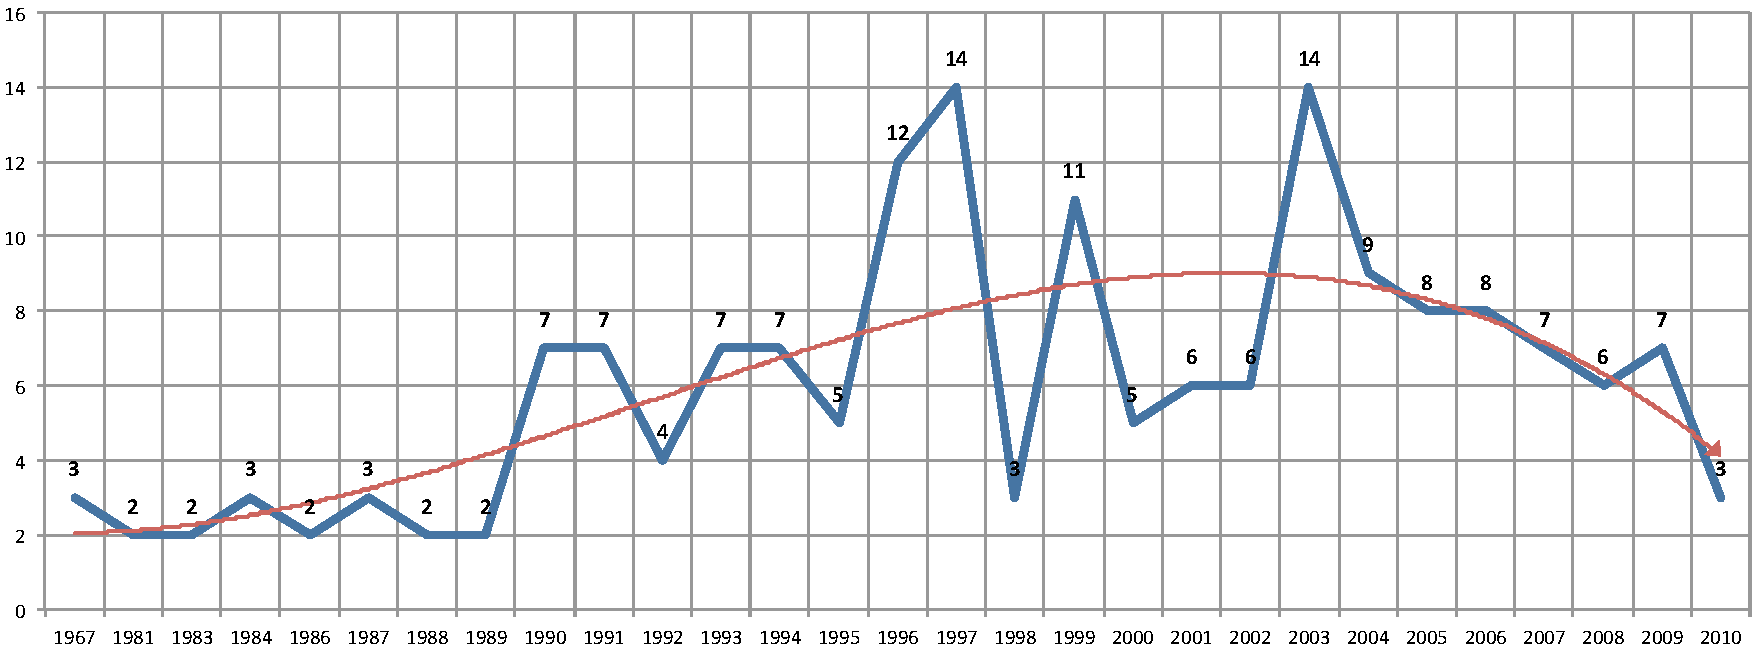
\includegraphics[scale=0.5]{img/abntex2-modelo-img-grafico}
  \end{center}
  \fonte{\citeonline[p. 24]{araujo2012}}
\end{figure}


A \autoref{fig:exemplo} na página \pageref{fig:exemplo} contém duas subfiguras, \autoref{subfig:exemplo:arquivo} e \subcaptionref{subfig:exemplo:tikz}.
  A \autoref{subfig:exemplo:arquivo} foi inserida de um arquivo externo, enquanto a \autoref{subfig:exemplo:tikz} foi escrita dentro do próprio código \TeX.
  A \autoref{fig:exemplo2} contém o mesmo exemplo, mas usando comandos diferentes para inserir as Subfiguras \ref{subfig:exemplo2:arquivo} e \subcaptionref{subfig:exemplo2:tikz}.

\begin{figure}[!htb]
  \centering
  \caption{Exemplo de subfiguras.}\label{fig:exemplo}
  \subbottom[Uma figura de um arquivo.]{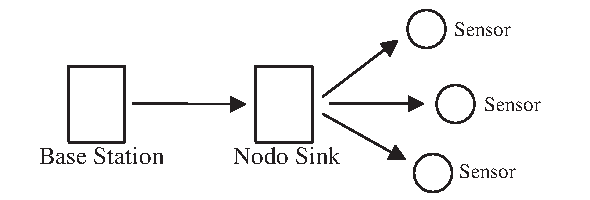
\includegraphics[scale=1]{img/exemplo}\label{subfig:exemplo:arquivo}}\fonte{\citeonline{Moro2012}}
  \qquad
  \subbottom[Uma figura em puro código TikZ.]{%
    \begin{tikzpicture}
      [tipo1/.style={rectangle,draw,minimum height=13mm,minimum width=9mm},
       tipo2/.style={circle,draw,minimum height=6mm,minimum width=6mm,
                     prefix after command={\pgfextra{\tikzset{every label/.style={font=\footnotesize}}}}},
       tiposeta/.style={->,shorten >=6pt,shorten <=6pt,>=triangle 60,thick}]
      \node [tipo1] (base) [label=below:Base Station] {};
      \node [tipo1] (sink) [right=22mm of base,label=below:Nodo Sink] {};
      \node [tipo2] (sensor1) [above right=4mm and 17mm of sink,label=right:Sensor] {};
      \node [tipo2] (sensor2) [right=22mm of sink,label=right:Sensor] {};
      \node [tipo2] (sensor3) [below right=4mm and 17mm of sink,label=right:Sensor] {};
      \draw [tiposeta] (base.east) -- (sink.west);
      \draw [tiposeta] (sink.east) -- (sensor1.south west);
      \draw [tiposeta] (sink.east) -- (sensor2.west);
      \draw [tiposeta] (sink.east) -- (sensor3.north west);
    \end{tikzpicture}
    \label{subfig:exemplo:tikz}%
  }
  \legend{Alterado: de \citeonline{Moro2012}}%
\end{figure}

Na \autoref{fig:exemplo}, as legendas (que indicam a fonte) para cada subfigura só funcionaram porque as figuras ficaram uma embaixo da outra.
  Se elas estivessem lado a lado, a inserção do comando \verb|\legend| em cada uma faria com que elas ficassem organizadas na vertical.
  Uma legenda geral funcionaria, entretanto.

Na \autoref{fig:exemplo2}, tanto legendas para subfiguras quanto uma legenda geral funcionam.

\begin{figure}[!htb]
  \centering
  \caption{Mesmo exemplo de subfiguras, agora em escala.}\label{fig:exemplo2}
  \begin{minipage}{0.48\textwidth}
    \centering
    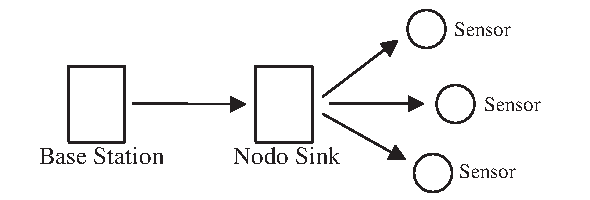
\includegraphics[scale=.5]{img/exemplo}
    \subcaption{Uma figura de um arquivo.\label{subfig:exemplo2:arquivo}}
    \fonte{\citeonline{Moro2012}}%
  \end{minipage}
  %\quad
  \begin{minipage}{0.48\textwidth}
    \centering
    \resizebox{0.6\textwidth}{!}{%
      \begin{tikzpicture}[%
         tipo1/.style={rectangle,draw,minimum height=13mm,minimum width=9mm},
         tipo2/.style={circle,draw,minimum height=6mm,minimum width=6mm,
                       prefix after command={\pgfextra{\tikzset{every label/.style={font=\footnotesize}}}}},
         tiposeta/.style={->,shorten >=6pt,shorten <=6pt,>=triangle 60,thick}]
        \node [tipo1] (base) [label=below:Base Station] {};
        \node [tipo1] (sink) [right=22mm of base,label=below:Nodo Sink] {};
        \node [tipo2] (sensor1) [above right=4mm and 17mm of sink,label=right:Sensor] {};
        \node [tipo2] (sensor2) [right=22mm of sink,label=right:Sensor] {};
        \node [tipo2] (sensor3) [below right=4mm and 17mm of sink,label=right:Sensor] {};
        \draw [tiposeta] (base.east) -- (sink.west);
        \draw [tiposeta] (sink.east) -- (sensor1.south west);
        \draw [tiposeta] (sink.east) -- (sensor2.west);
        \draw [tiposeta] (sink.east) -- (sensor3.north west);
      \end{tikzpicture}
    }
    \subcaption{\label{subfig:exemplo2:tikz}Uma figura em puro código TikZ.}
    \fonte{Alterado de \citeonline{Moro2012}}%
  \end{minipage}
  \fonte{Fonte geral}%
\end{figure}


%------------------------------------------------------------------------------
\subsection{Sobre a indicação da fonte de uma tabela ou figura}
%------------------------------------------------------------------------------

As normas \citeonline[5.8]{NBR14724:2011} e o Manual de Normatização da UNIPAMPA \cite{SisbiUnipampa2011} dizem para, ``Após a ilustração, na parte inferior, indicar a fonte consultada (elemento obrigatório, mesmo que seja produção do próprio autor), legenda, notas e outras informações necessárias à sua compreensão (se houver).''
  A primeira interpretação é a de que, mesmo que o autor tenha criado a figura, a fonte deverá ser indicada.
  Com efeito, várias outras normas, manuais e inclusive o exemplo do pacote \abnTeX2 usam ``Fonte: os autores'' em alguns lugares.

Entretanto, isso não está correto.
  Veja o trecho em destaque: ``Após a ilustração, na parte inferior, indicar a fonte \textbf{consultada} (elemento obrigatório, mesmo que seja produção do próprio autor) (...).''
  A interpretação correta é a de que, caso a ilustração tenha sido \textbf{extraída} de um documento, a fonte deve ser indicada, ainda que esse documento pertença ao próprio autor.
  A sentença original das normas deveria ter sido melhor escrita para evitar a interpretação incorreta.

Assim, não indique a fonte se a figura ou tabela for original, ou seja, foi criada para o trabalho.
  Caso contrário, indique a fonte.
  Mas cuidado: caso a figura ou tabela tenha sido adaptada de outra já publicada, então é obrigatório indicar ``adaptado de'' ou ``acrescida de'' seguido da referência da fonte de onde ela foi extraída.


%------------------------------------------------------------------------------
\section{Expressões matemáticas}
%------------------------------------------------------------------------------

\index{expressões matemáticas}Use o ambiente \texttt{equation} para escrever expressões matemáticas numeradas:

\begin{equation}
  \forall x \in X, \quad \exists \: y \leq \epsilon
\end{equation}

Escreva expressões matemáticas entre \$ e \$, como em $\lim_{x \to \infty} \exp(-x) = 0$, para que fiquem na mesma linha.

Também é possível usar colchetes para indicar o início de uma expressão matemática que não é numerada.

\[
\left|\sum_{i=1}^n a_ib_i\right|
\le
\left(\sum_{i=1}^n a_i^2\right)^{1/2}
\left(\sum_{i=1}^n b_i^2\right)^{1/2}
\]

Consulte mais informações sobre expressões matemáticas em \url{http://code.google.com/p/abntex2/w/edit/Referencias}.


%------------------------------------------------------------------------------
\section{Enumerações: alíneas e subalíneas}
%------------------------------------------------------------------------------

\index{alíneas}\index{subalíneas}\index{incisos}Quando for necessário enumerar os diversos assuntos de uma seção que não possua título, esta deve ser subdividida em alíneas \cite[4.2]{NBR6024:2012}:

\begin{alineas}

  \item os diversos assuntos que não possuam título próprio, dentro de uma mesma
  seção, devem ser subdivididos em alíneas\footnote{As notas devem ser digitadas ou datilografadas
  dentro das margens, ficando separadas do texto por um espaço simples de entre as
  linhas e por filete de 5 cm, a partir da margem esquerda. Devem ser
  alinhadas, a partir da segunda linha da mesma nota, abaixo da primeira letra
  da primeira palavra, de forma a destacar o expoente, sem espaço entre elas e
  com fonte menor. \citeonline[5.2.1]{NBR14724:2011}};

  \item o texto que antecede as alíneas termina em dois pontos;
  \item as alíneas devem ser indicadas alfabeticamente, em letra minúscula, seguida de parêntese. Utilizam-se letras dobradas, quando esgotadas as letras do alfabeto;

  \item as letras indicativas das alíneas devem apresentar recuo em relação à
  margem esquerda;

  \item o texto da alínea deve começar por letra minúscula e terminar em
  ponto-e-vírgula, exceto a última alínea que termina em ponto final;

  \item o texto da alínea deve terminar em dois pontos, se houver subalínea;

  \item a segunda e as seguintes linhas do texto da alínea começa sob a
  primeira letra do texto da própria alínea;

  \item subalíneas \cite[4.3]{NBR6024:2012} devem ser conforme as alíneas a
  seguir:

  \begin{alineas}
     \item as subalíneas devem começar por travessão seguido de espaço;

     \item as subalíneas devem apresentar recuo em relação à alínea;

     \item o texto da subalínea deve começar por letra minúscula e terminar em
     ponto-e-vírgula. A última subalínea deve terminar em ponto final, se não
     houver alínea subsequente;

     \item a segunda e as seguintes linhas do texto da subalínea começam sob a
     primeira letra do texto da própria subalínea.
  \end{alineas}

  \item no \abnTeX\ estão disponíveis os ambientes \texttt{incisos} e \texttt{subalineas}, que em suma são o mesmo que se criar outro nível de \texttt{alineas}, como nos exemplos à seguir:

  \begin{incisos}
    \item \textit{Um novo inciso em itálico};
  \end{incisos}

  \item Alínea em \textbf{negrito}:

  \begin{subalineas}
    \item \textit{Uma subalínea em itálico};
    \item \underline{\textit{Uma subalínea em itálico e sublinhado}};
  \end{subalineas}

  \item Última alínea com \emph{ênfase}.

\end{alineas}


%------------------------------------------------------------------------------
\section{Espaçamento entre parágrafos e linhas}
%------------------------------------------------------------------------------

\index{espaçamento!dos parágrafos}O tamanho do parágrafo, espaço entre a margem e o início da frase do parágrafo, é definido por:

\begin{verbatim}
   \setlength{\parindent}{1.3cm}
\end{verbatim}

\index{espaçamento!do primeiro parágrafo}Por padrão, não há espaçamento no primeiro parágrafo de cada início de divisão do documento (\autoref{sec:divisoes}).
  Porém, você pode definir que o primeiro parágrafo também seja indentado, como é o caso deste documento.
  Para isso, apenas inclua o pacote \textsf{indentfirst} no preâmbulo do documento:
\begin{verbatim}
   \usepackage{indentfirst}      % Indenta o primeiro parágrafo de cada seção.
\end{verbatim}

\index{espaçamento!entre os parágrafos}O espaçamento entre um parágrafo e outro pode ser controlado por meio do comando:
\begin{verbatim}
  \setlength{\parskip}{0.2cm}  % tente também \onelineskip
\end{verbatim}

\index{espaçamento!entre as linhas}O controle do espaçamento entre linhas é definido por:
\begin{verbatim}
  \OnehalfSpacing       % espaçamento um e meio (padrão);
  \DoubleSpacing        % espaçamento duplo
  \SingleSpacing        % espaçamento simples
\end{verbatim}

Para isso, também estão disponíveis os ambientes:
\begin{verbatim}
  \begin{SingleSpace} ...\end{SingleSpace}
  \begin{Spacing}{hfactori} ... \end{Spacing}
  \begin{OnehalfSpace} ... \end{OnehalfSpace}
  \begin{OnehalfSpace*} ... \end{OnehalfSpace*}
  \begin{DoubleSpace} ... \end{DoubleSpace}
  \begin{DoubleSpace*} ... \end{DoubleSpace*}
\end{verbatim}

Para mais informações, consulte \citeonline[p. 47-52 e 135]{memoir}.


%------------------------------------------------------------------------------
\section{Inclução de outros arquivos}\label{sec:include}
%------------------------------------------------------------------------------

É uma boa prática dividir o seu documento em diversos arquivos, e não apenas escrever tudo em um único.
  Esse recurso foi utilizado neste documento.
  Para incluir diferentes arquivos em um arquivo principal, de modo que cada arquivo incluído fique em uma página diferente, utilize o comando:
\begin{verbatim}
   \include{documento-a-ser-incluido}      % sem a extensão .tex
\end{verbatim}

Para incluir documentos sem quebra de páginas, utilize:
\begin{verbatim}
   \input{documento-a-ser-incluido}      % sem a extensão .tex
\end{verbatim}


%------------------------------------------------------------------------------
\section{Compilar o documento \LaTeX}
%------------------------------------------------------------------------------

Geralmente os editores \LaTeX, como o TeXlipse\footnote{\url{http://texlipse.sourceforge.net/}}, o Texmaker\footnote{\url{http://www.xm1math.net/texmaker/}}, entre outros, compilam os documentos automaticamente, de modo que você não precisa se preocupar com isso.

No entanto, você pode compilar os documentos \LaTeX usando os seguintes comandos, que devem ser digitados no \emph{Prompt de Comandos} do Windows ou no \emph{Terminal} do Mac ou do Linux:
\begin{verbatim}
   pdflatex ARQUIVO_PRINCIPAL.tex
   bibtex ARQUIVO_PRINCIPAL.aux
   makeindex ARQUIVO_PRINCIPAL.idx
   makeindex ARQUIVO_PRINCIPAL.nlo -s nomencl.ist -o ARQUIVO_PRINCIPAL.nls
   pdflatex ARQUIVO_PRINCIPAL.tex
   pdflatex ARQUIVO_PRINCIPAL.tex
\end{verbatim}
 % [OBRIGATORIO]
%\part{Resultados}
%\input{textuais/outrospontos} % Outro capítulo
%\bookmarksetup{startatroot} % Usar se o próximo capítulo não pertencer à parte anterior e não existir uma parte nova
%==============================================================================
\chapter{Considerações Finais}\label{conclusao}
%==============================================================================

Em Trabalhos de Conclusão de Curso, use ``\emph{Considerações Finais}'' e não ``\emph{Conclusão}''.

Bom trabalho!
 % [OBRIGATORIO]


% +++++++++++++++++++++++++++++++++++++++++++++++++++++++++++++++++++++++++++++++++++++++++++++++++
% ELEMENTOS PÓS-TEXTUAIS
% +++++++++++++++++++++++++++++++++++++++++++++++++++++++++++++++++++++++++++++++++++++++++++++++++
\postextual

% -----------------------------------------------
% Bibliografia [OBRIGATORIO]
% -----------------------------------------------
% Nome(s) do(s) arquivo(s) .bib (sem a extensão)
\bibliography{bibliografia,abntex2-modelo-references}

% -----------------------------------------------
% Apêndices [OPCIONAL]
% -----------------------------------------------
\begin{apendicesenv}

% Imprime uma página indicando o início dos apêndices
\partapendices

% Para cada apêndice, um \chapter


%==============================================================================
\chapter{Primeiro Apêndice}
%==============================================================================

De acordo com a ABNT:

\begin{quotation}
Apêndice (opcional): texto utilizado quando o autor pretende complementar sua argumentação. São identificados por letras maiúsculas e travessão, seguido do título. Ex.: APÊNDICE A - Avaliação de células totais aos quatro dias de evolução

Anexo (opcional): texto ou documento \textbf{não elaborado pelo autor} para comprovar ou ilustrar. São identificados por letras maiúsculas e travessão, seguido do título. Ex.: ANEXO A - Representação gráfica de contagem de células
\end{quotation}

Tais definições (e outras) podem ser encontradas na NBR 14724-2001 Informação e documentação - trabalhos acadêmicos\footnote{http://www.firb.br/abntmonograf.htm}.


%==============================================================================
\chapter{Segundo Apêndice}
%==============================================================================

Pode ser que tenha outro...


\end{apendicesenv}


% -----------------------------------------------
% Anexos [OPCIONAL]
% -----------------------------------------------
\begin{anexosenv}

% Imprime uma página indicando o início dos anexos
\partanexos

% Para cada anexo, um \chapter


%==============================================================================
\chapter{Primeiro Anexo}
%==============================================================================

Sendo anexo, a formatação dessa seção é livre. Ou seja: aceita-se fonte diferente e menor


%==============================================================================
\chapter{LaTex para Principiantes}\label{anexo:latex}
%==============================================================================
TEste\footnote{\cite{Moro2012}}
Dentro dos arquivos .tex o texto pode estar organizado em partes, capítulos, seções, etc. conforme os seguintes comandos:

-- \verb|\part{NomedaParte}|, partes do documento \\
-- \verb|\chapter{Nome}|, capítulos somente para arquivos do tipo \textit{book} e \textit{report}\\
-- \verb|\section{Nome}|, seções\\
-- \verb|\subsection{Nome}|, subseções	\\
-- \verb|\subsubsection{Nome}|, seções dentro de subseções\\
-- \verb|\paragraph{Texto}|, parágrafos formatados	\\
-- \verb|\subparagraph{Texto}|, subparágrafos

\textbf{Parágrafos} Parágrafos são definidos deixando uma linha em branco entre os mesmos.
  Pode-se também forçar usando \verb|\\| bem como deixar uma linha em branco com um \verb|~| sozinho na linha.

\textbf{Formato de texto} O tamanho do texto pode ser definido pelos comandos específicos:  \verb|tiny|,  \verb|scriptsize|,  \verb|footnotesize|, \verb|small|, \verb|normalsize|, \verb|large|, \verb|Large|, \verb|huge| e \verb|Huge|, conforme ilustra a Figura \ref{fig:fontsize}\todo{Perceba que a figura tem resolução ruim; deveria ser uma tabela}.

\begin{figure}[ht]
	\centering
		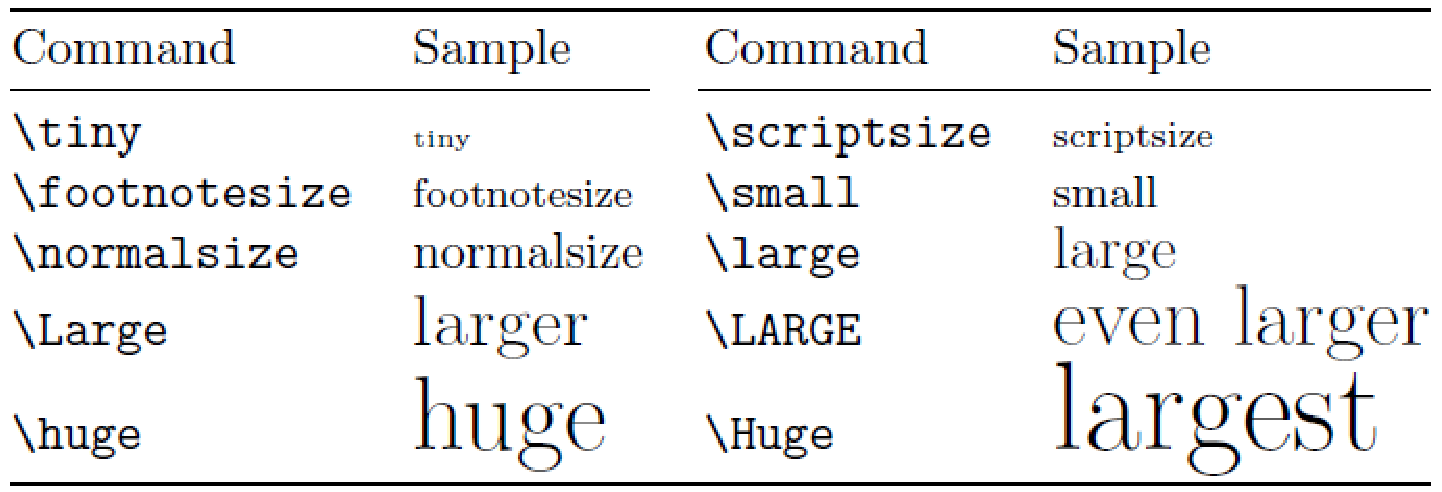
\includegraphics[width=0.7\textwidth]{img/fontsize}
	\caption{Exemplo de tamanhos de fonte}
	\label{fig:fontsize}
\end{figure}

\textbf{Referências dentro do Texto} Partes do texto podem ser referenciadas através do par de comandos \verb|\label| e \verb|\ref|.
  Por exemplo, podemos inserir uma seção no artigo utilizando o seguinte comando:

\begin{verbatim}
\section{Seção principal}\label{sec:prcpal}
\end{verbatim}

Vejam que o título da seção é seguido do comando \verb|\label{nome}|.
  Esta seção pode ser referenciada em qualquer parte do texto, como o exemplo a seguir.

\begin{verbatim}
Conforme explicado na Seção \ref{sec:prcpal}, nosso método utiliza...
\end{verbatim}


%------------------------------------------------------------------------------
\section{Outras Dicas}
%------------------------------------------------------------------------------

\textbf{Caracteres Especiais} Esses não podem ser usados no texto sem a barra à frente: \# \$ \% \^{ } \& \_ \{ \} \~{ } e \slash .

\textbf{Comentários} Comentários são precedidos de \% e podem estar em qualquer parte do texto.
  Lembrando que tudo que estiver após \% será considerado como comentário e ignorado pelo processador.

\textbf{Incluir Figuras} Incluir figuras no LaTeX é relativamente fácil quando se tem um formato de arquivo pré-definido.
  or exemplo, neste documento, usa-se apenas figuras do tipo \textit{pdf}, mas também poderia-se usar do tipo \textit{png} (e \textit{jpeg}, mas este tipo não é recomendado).
  A Tabela \ref{tab:codfig} ilustra as linhas que inserem uma figura no texto. 

\begin{table}[ht]
  \caption{Linhas de código para inserir figura}
	\centering
	\footnotesize	
		\begin{tabular}{l l}
	\\	\hline 
Linha de Código & Explicação \\ \hline 
\verb|\usepackage{graphicx}| & \textit{inclui pacote gráfico no início do documento} \\
\verb|\begin{figure}[tb]|    & \textit{inicia figura, define sua posição no texto} \\
\verb|\centering|            & \textit{centraliza a figura na página}\\
\verb|\includegraphics[scale=.7]|& \textit{define escala da figura}\\
\verb|{img/figura}|      & \textit{inclui o arquivo da figura no texto}\\
\verb|\caption{Legenda}|     & \textit{inclui a legenda da figura}\\
\verb|\label{fig:ap}|        & \textit{inclui o apelido da figura}\\
\verb|\end{figure}|          & \textit{termina figura}\\
		\hline\end{tabular}
	\label{tab:codfig}
\end{table}

\textbf{Hifenização} Às vezes aparece uma palavra cuja hifenização, divisão silábica, está errada. Para resolver esse tipo de problema, pode-se recorrer à divisão manual da palavra, acrescentando \verb|\-| entre cada sílaba: \verb|Mi\-re\-lla|. Se, ao invés desta solução, você quiser evitar completamente que suas palavras sejam divididas, acrescente os dois comandos no início do seu documento (ou seja, antes do \\~\textit{begin\{document\}}).

\begin{verbatim}
  \hyphenpenalty=5000
  \tolerance=1000
\end{verbatim}


\textbf{BibTeX} Para editar facilmente o BibTeX, pode-se utilizar uma ferramenta própria\footnote{Ferramentas para BibTeX: http://dmoz.org/Computers/Software/Typesetting/TeX/BibTeX}. A minha favorita é o JabRef\footnote{JabRef Editor: http://jabref.sourceforge.net/}, ilustrado na Figure \ref{fig:jabref}, porque:

\begin{itemize}\addtolength{\itemsep}{-0.5\baselineskip}
	\item É de graça;
	\item Possui interface gráfica super intuitiva;
	\item Permite importar referências de bases clássicas, como ISI, Medline e RIS;
	\item Permite exportar para diferentes formatos, inclusive para um banco de dados utilizando SQL;
	\item Tem botão para procurar o artigo da respectiva referência e fazer o seu download;
	\item Permite adicionar comentários próprios para cada entrada;
	\item Pode-ser classificar as referências e criar grupos para as mesmas, e muito muito mais.
\end{itemize}

\begin{figure}[tb]
	\centering
		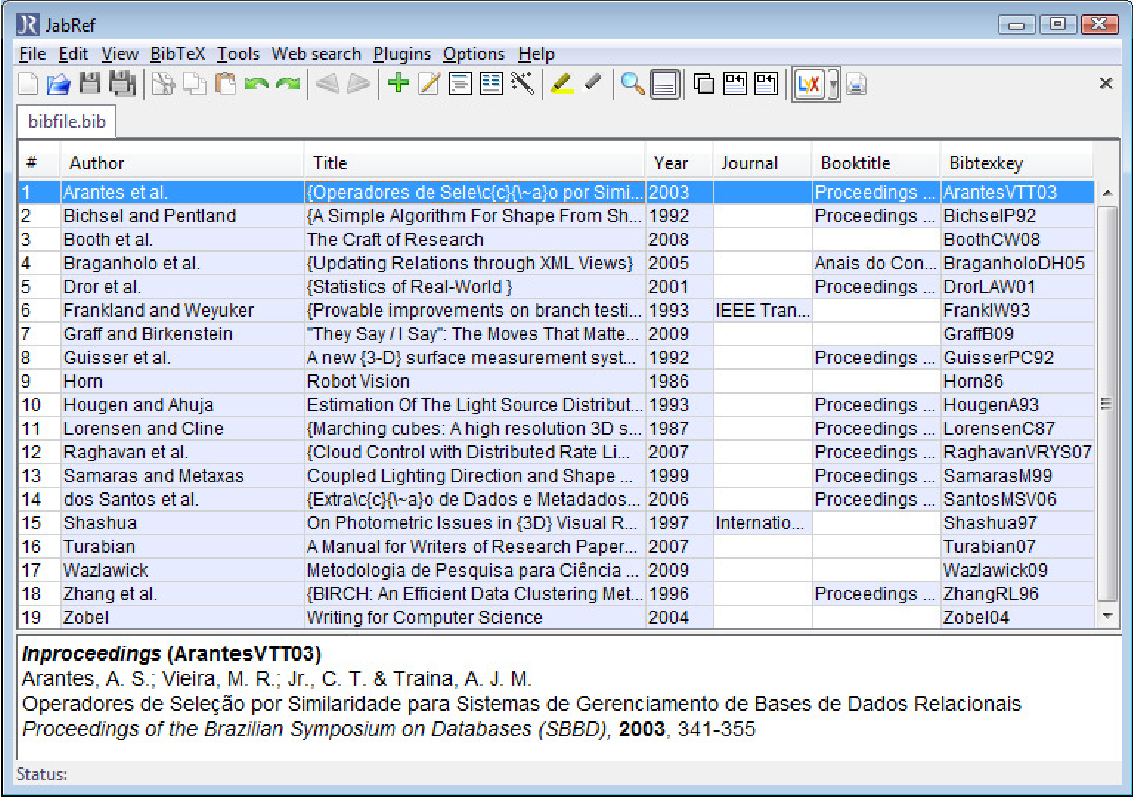
\includegraphics[width=0.98\textwidth]{img/jabref}
	\caption{Tela do JabRef para uma versão inicial do arquivo bib deste documento}
	\label{fig:jabref}
\end{figure}

\textbf{Listas} Listas podem ser definidas com \textit{bullets} ou com números, conforme os exemplos a seguir.

\begin{verbatim}
\begin{itemize}
\item Item 1 com bullet 
\item Item 2 com bullet 
\end{itemize}

\begin{enumerate}
	\item Item 1 numerado
	\item Item 2 numerado
\end{enumerate}
\end{verbatim}

\textbf{Fontes Coloridas} Para adicionar texto em cores (muito útil para marcar trechos do texto que estão \textit{em trabalho}, deve-se adicionar os pacotes \textit{graphicx} e \textit{color} (usando o comando \verb|\usepackage| e depois utilizar o comando \verb|\textcolor{cor}{texto}| para colorir o \textit{texto} com a \textit{cor} especificada. Por exemplo \verb|\textcolor{blue}{texto em azul}|. Outras cores comuns são \textit{red} e \textit{green}.

\textbf{Para Economizar Espaço} Existem alguns \textit{dirty tricks}\footnote{Ou seja, eles irão alterar a formatação dada pelo estilo default do texto.} pra economizar espaço, como por exemplo:

-- \verb|\usepackage{times}| Usa fonte \textit{Times} no lugar da default.

-- \verb|\usepackage[small,compact]{titlesec}| Modifica o título e os espaços antes/depois dos mesmos.

-- \verb|\usepackage[small,it]{caption}| Reduz o tamanho das legendas de tabelas e figuras.

\textbf{WEB} A Web é repleta de páginas e documentos sobre LaTeX. Alguns exemplos incluem:

\begin{itemize}\addtolength{\itemsep}{-0.5\baselineskip}
  \item Favorito inglês: \url{http://en.wikibooks.org/wiki/LaTeX/}
  \item Favorito português: \url{http://linorg.usp.br/CTAN/info/lshort/portuguese/pt-lshort.pdf}
  \item \url{http://www.mat.ufmg.br/~regi/topicos/intlat.pdf}
  \item \url{http://www.duke.edu/~hg9/ctex/LaTeXManual.pdf}
  \item \url{http://minerva.ufpel.tche.br/~campani/cursolatex.pdf}
	\item \url{http://www.personal.ceu.hu/tex/words.htm}
\end{itemize}


\end{anexosenv}


% -----------------------------------------------
% Índice Remissivo [OPCIONAL]
% -----------------------------------------------
% Veja o pacote makeindex para mais informações
\printindex


\end{document}
